\documentclass[varwidth,border=7mm]{standalone}
\usepackage{tikz}
\usetikzlibrary{decorations.pathreplacing}
\usetikzlibrary{arrows.meta}
\usetikzlibrary{calc}
\tikzset{
  yl/.style={inner sep=1pt,fill=white,font=\small\tt,text=orange},
  xl/.style={inner sep=1pt,font=\small\tt,blue,below},
  dl/.style={inner sep=1pt,font=\small\tt,purple},
  pt/.style={node contents=.,text=black,scale=1.5}
}
\begin{document}
  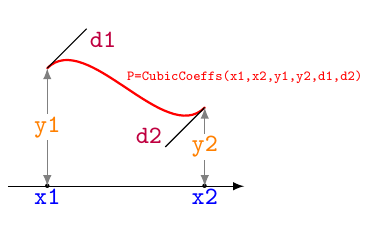
\begin{tikzpicture}
    \coordinate (O);
    \coordinate (A) at (0,1.5);
    \coordinate (B) at (2,1);
    \coordinate (DA) at (.5,.5);
    \coordinate (DB) at (-.5,-.5);
    \draw[red,thick,line cap=round] (A) .. controls +(DA) and +(DB) .. node[yshift=4pt,right,inner sep=0pt,font=\tiny\tt]{P=CubicCoeffs(x1,x2,y1,y2,d1,d2)}(B);
    \draw (A) -- +(DA) node[dl,below right]{d1} (B) -- +(DB) node[dl,above left]{d2};
    \draw[shorten <=-5mm, shorten >= -5mm, -latex] (A|-O) node[xl]{x1} node[pt]{} -- (B|-O) node[xl]{x2} node[pt]{};
    \draw[gray,latex-latex] (A|-O)  -- node[yl]{y1} (A);
    \draw[gray,latex-latex] (B|-O)  -- node[yl]{y2} (B);
  \end{tikzpicture}
\end{document}
